\documentclass[12pt,letterpaper]{article}

\author{Jordan Bayles}

%Usepackage declarations
\usepackage[left=1in,top=1in,right=1in,bottom=1in]{geometry}
%\usepackage[T1]{fontenc}
%\usepackage{tgpagella}
%\usepackage[protrusion=true,expansion=true]{microtype}
\usepackage{xcolor}
\usepackage{color}
\usepackage{fancyhdr}
\usepackage{lastpage}
\usepackage{sectsty}
\usepackage{slashed}
\usepackage{amsmath}
\usepackage{amsfonts}
\usepackage{listings}
\usepackage{latexsym}
% Include for easy import of full pdf pages
\usepackage{pdfpages}
% Include for use of images
\usepackage{graphicx}
% Include for use of [H] placement specifier
\usepackage{float}
% Include for use of \toprule, \midrule, \bottomrule in tabular env.
\usepackage{booktabs}
% Include for setting spacing between lines
\usepackage{setspace}

%Package usages
\sectionfont{\normalsize}
\subsectionfont{\small}

%%Fancy Header setup
\pagestyle{fancy}
% Clear default
\fancyhead{}
\fancyfoot{}
%New settings
\fancyhead[LE,RO]{\slshape \rightmark}
\fancyhead[LO,RE]{\slshape \leftmark}
\fancyfoot[C]{\thepage}
\renewcommand{\headrulewidth}{0.4pt}
\renewcommand{\footrulewidth}{0.4pt}

%New commands
\newcommand{\comment}[1]{}
\newcommand{\field}[1]{\mathbb{#1}} % requires amsfonts
\newcommand{\script}[1]{\mathcal{#1}} % requires amsfonts
\newcommand{\pd}[2]{\frac{\partial#1}{\partial#2}}

\begin{document}
%\maketitle

\begin{flushright}
Jordan Bayles\\
Data Structures (CS 261)\\
Ron Metoyer\\
\today
\end{flushright}

\begin{center}
Problem 2 - Comparison
\end{center}

\begin{figure}[H]
    \centering
    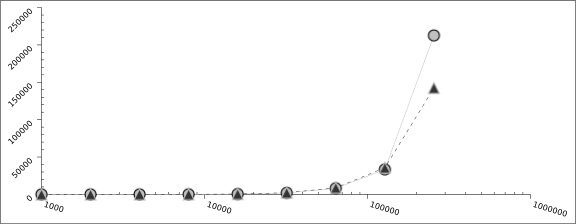
\includegraphics[width=6in]{graph.png}
    \caption{Graph comparison of runtimes for different data types}
\end{figure}

\section{Questions}
\subsection{ Which of the implementations is the fastest? }
They appear to be both be of similar run times. Judging by the
fact that they both have to iterate through the data set
(the dynamic array and the linked list both have to inspect each
element to determine its value), and we are merely checking the
content instead of adding or removing it, the implementation
difference should be small and they should both be $\mathcal{O}(n)$
for linear time operations. However, it does appear the linked list
begins to take more time for larger values, although they remain
fairly similar.

\subsection{ Would you expect anything to change if the loop performed
\texttt{remove()} instead of \texttt{contains()}? If so, what? }
It would have a significant impact on running time, as each element
would take incrementally less time to find (both contains and remove
must locate the element first), so both the linked list and
dynamic array would take noticeably less time than they do currently.
I would expect the linked list to take slightly less time due to the fact that
the dynamic array has to resize itself during operation.

\end{document}
